\documentclass{llncs}
\usepackage{graphicx}

\begin{document}
%
% --\item Author Metadata here ---
\conferenceinfo{WWW}{'15}
%\CopyrightYear{2007} % Allows default copyright year (20XX) to be over-ridden \item IF NEED BE.
%\crdata{0-12345-67-8/90/01}  % Allows default copyright data (0-89791-88-6/97/05) to be over-ridden \item IF NEED BE.
% --\item End of Author Metadata ---

\title{The Dynamics of Micro-task Crowdsourcing -- The Case of MTurk}
% anatomy of a Micro-task Crowdsourcing platform
% unravelling micro-task crowdsourcing dynamics/processes
% the evolution of micro-task crowdsourcing



%\numberofauthors{1}
\author{}

\maketitle
\begin{abstract}
Micro-task crowdsourcing is gaining popularity among serval organizations and research corps to leverage Human Computation in their daily operations. Unlike any other ``technology'', a crowdsourcing platform is subject to many factors that affect the performance, both in terms of speed and quality, of its services. Indeed, such factors shape the \emph{dynamics} of the market. For example, a common result is that increasing the price of a HIT would lead to faster results, however, we still do not know the exact impact of changing the price in the presence of many reputable requesters on the platform. Or, what happen when you post a link of a batch on a popular crowdsourcing forum etc.

In this paper we adopt a data-driven approach to analyze the behavior of the main actors in MTurk micro-task crowdsourcing: workers, requesters, HITs, and platform (MTurk); thanks to a collection of datasets that we gathered during the last X year.

The ultimate contribution that we propose is a predictive model to derive the expected performance of a published batch of HITs on MTurk at a specific moment in time.

\end{abstract}

A category with the (minimum) three required fields
\category{H.4}{Information Systems Applications}{Miscellaneous}
%A category including the fourth, optional field follows...
% \category{D.2.8}{Software Engineering}{Metrics}[complexity measures, performance measures]

\terms{Design, Experimentation, Human Factors}

\keywords{Crowdsourcing, social networks, log analysis}


\section{Datasets}
We leverage the data that we collected from the following sources:
\begin{itemize}
	\item Data from Mechanical Turk Tracker (TR)
	\item Data about requester reputation from Turkopticon (TO)
	\item Data from OpenTurk \footnote{A Chrome extension we have developed, see bit.ly/openturk-extension, It has 400+ users and been running since Feb, 2014.}
	\item Data from forums (e.g., mturkforum.com) about shared HITs. (FO)
	\item Data from surveys run on MTurk asking about worker experience and preferred tools (SU)
\end{itemize}


\section{Research Questions}

Possible research questions we want to answer and common assumptions we want to validate in a data-driven manner are:
(Organized by market actor)

\subsection{Requesters}
\begin{itemize}
	\item How does a good requester reputation affects the latency of HIT? 
	For example, is the common assumption that generous requesters obtain lower latency correct at large scale? (TO, TR)
	\item How do requesters republish HITs or extend HIT lifetime to attract additional workforce?
\end{itemize}


\subsection{Workers}
\begin{itemize}
	\item How much time do workers spend to search/find the next HIT batch to work on? (OT)
	\item Does share activity on worker social media trigger an increased throughput (measured in HIT/min) of the HIT batch? (FO, OT, TR)
	\item Do the number of followers on OpenTurk correlate with requester reputation? (TO,OT) -- See Figure \ref{fig:figure2} for early results.
\end{itemize}


\paragraph{Platform}
\begin{itemize}
	\item How has the requester set size evolved over time? (TR)
	\item How HITs from top requesters affect rewards and latency of other batches concurrently running on the platform? (TO,OT,TR)
	-- See Figure \ref{fig:figure1} for current state of affairs -- big batches take all the attention (assuming that we are not missing many data points in the intra 20min crawl-window).
\end{itemize}

\paragraph{HITs}
\begin{itemize}
	\item Which are the different categories of HITs published on MTurk? We plan to define a taxonomy of common HITs including classification, survey, translation, typing, etc.
	\item Using the taxonomy, how does reward and completion time vary with HIT type? (TR, OT)
	\item How has the average reward evolved over time for each HIT type? (TR)
	\item How has the average throughput (measured in HIT/min) evolved over time for each HIT type? (TR)
\end{itemize}

\section{Model of The Market}
As a result of the previous analysis, we would like to propose a formal model of the throughput obtained by a certain requester publishing a HIT batch in certain conditions taking into consideration aspects like: requester reputation (TO), HIT social media visibility (FR,OT), task type (taxonomy), reward (TR).

\section{Early Results}
All this could sound ambitious, but we have already started putting hands on the data. For example, the attached Figure 1 shows HIT batch throughput as compared to HIT batch size over 3 months of TR data and Figure 2 shows the correlation of a requester followers on OT with requester reputation on TO using different metrics and composition of metrics (more TOS reduces the number of followers, while requesters with more reviews are followed more).

\begin{figure}[htbp]
	\centering
		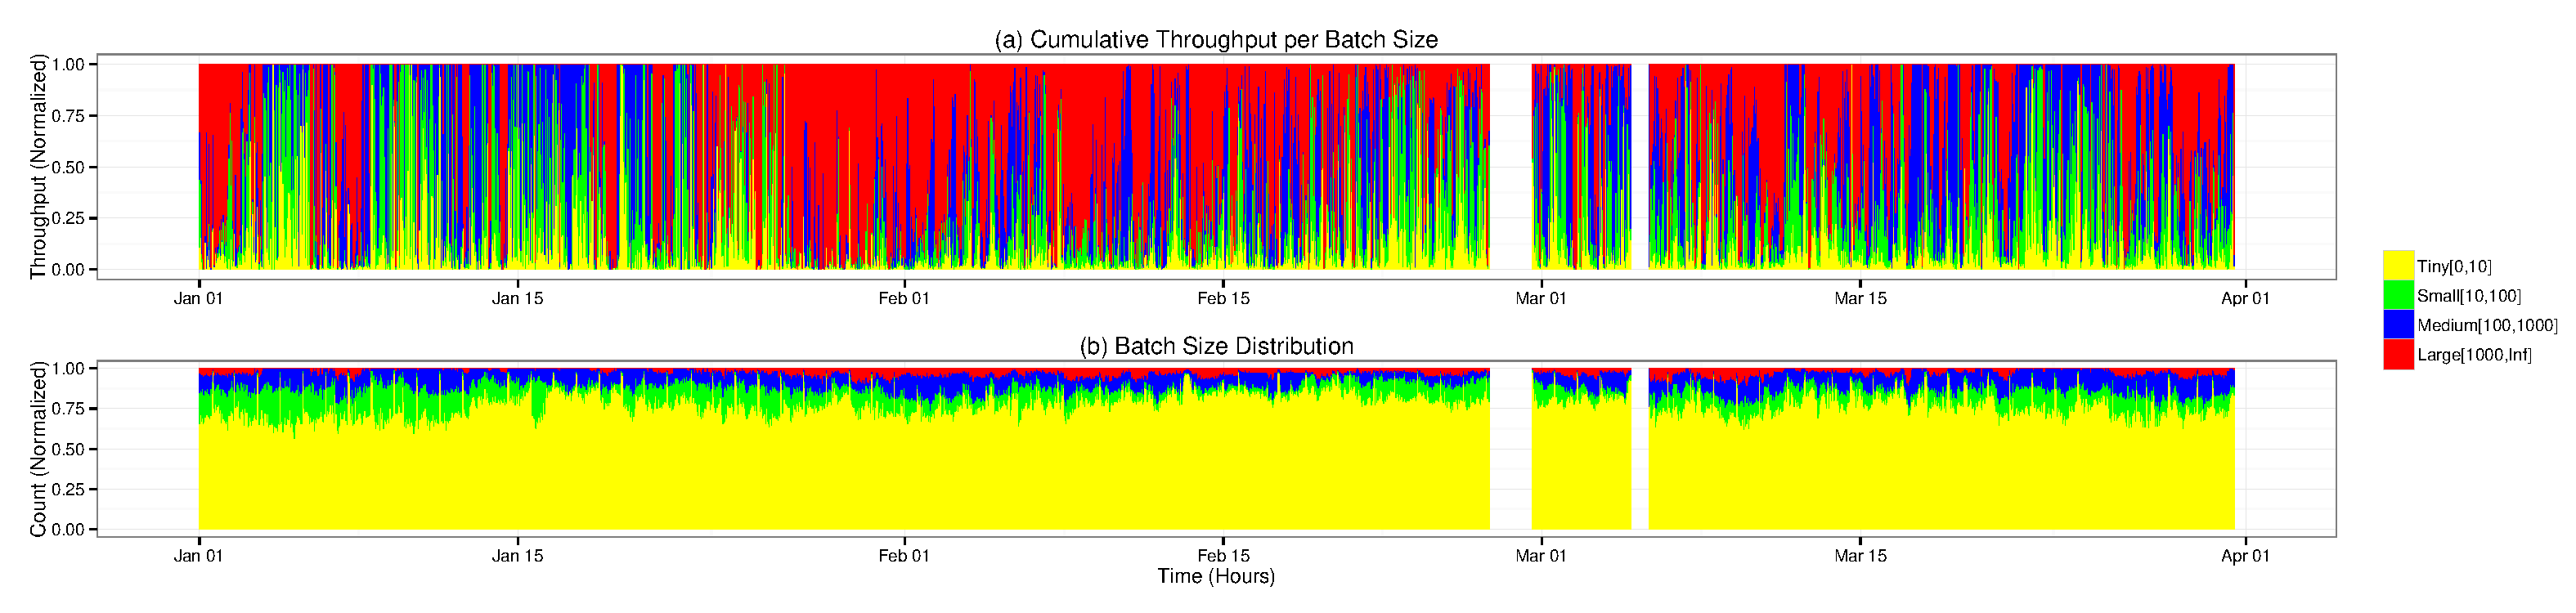
\includegraphics[width=1.2\textwidth]{figures/analysis_hour}
	\caption{HIT batch throughput as compared to HIT batch size over 3 months of TR data. The majority of the workforce is geared toward the big batch (this results is used in another piece of our work), still most of the batches on the platform are small sized.}
	\label{fig:figure1}
\end{figure}

\begin{figure}[htbp]
	\centering
		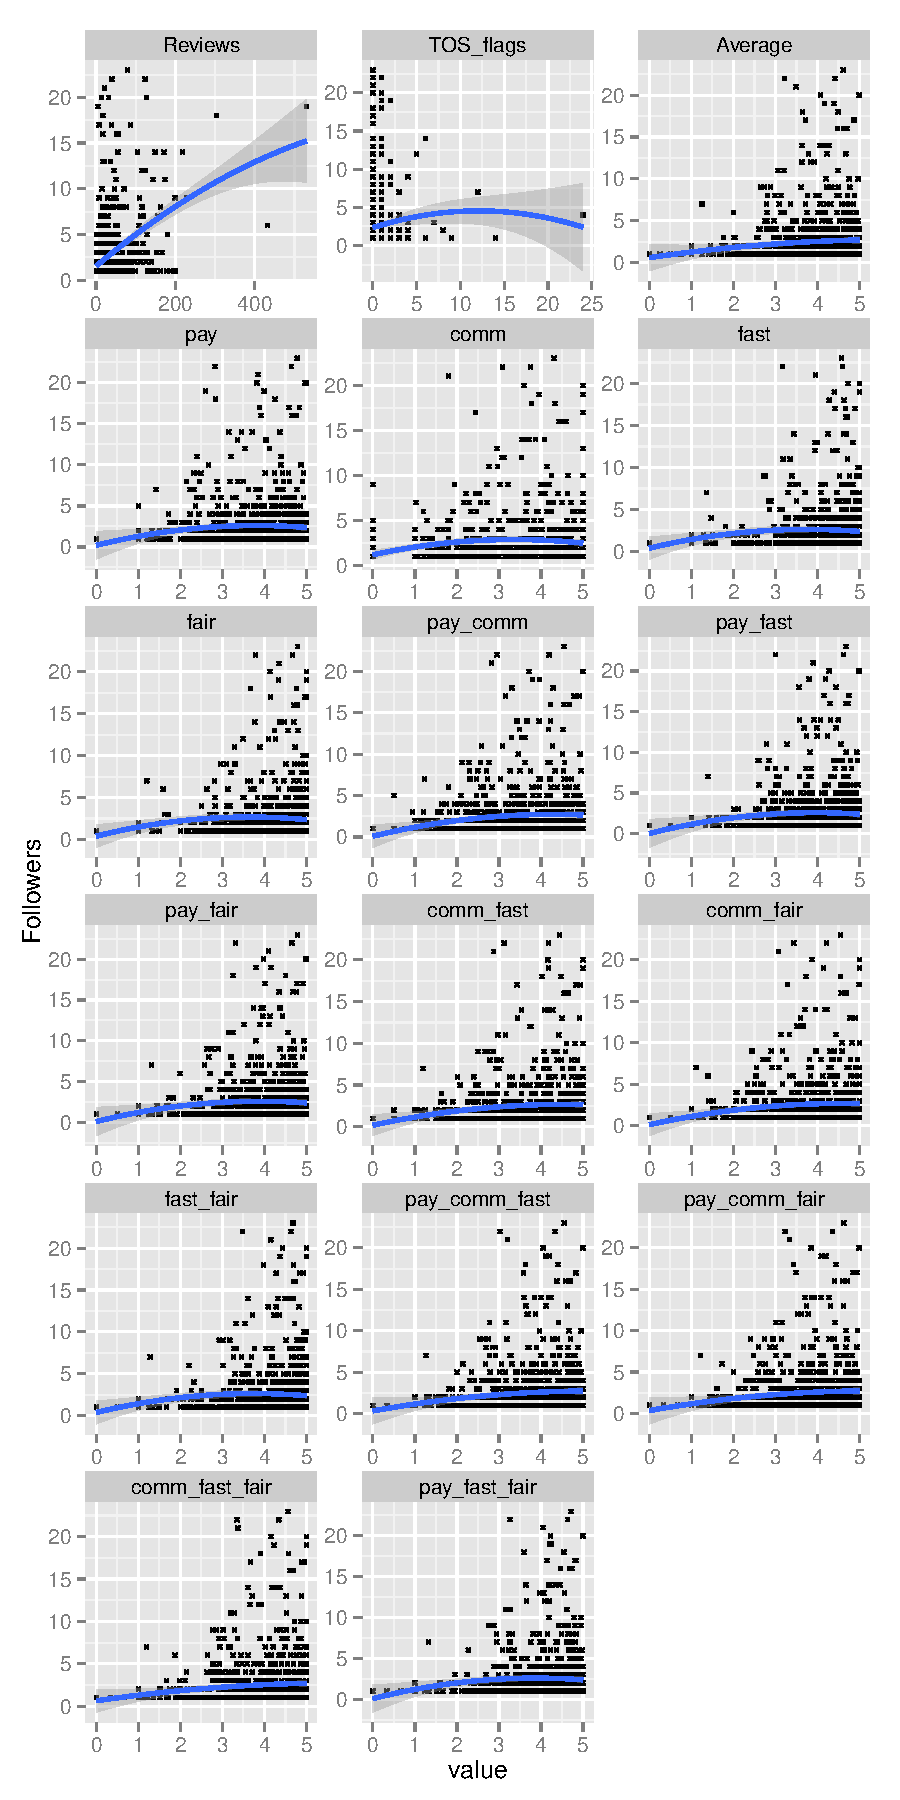
\includegraphics[width=0.9\textwidth]{figures/correlation}
	\caption{Correlation of a requester followers on OT with requester reputation on TO.}
	\label{fig:figure2}
\end{figure}

\end{document}
